\documentclass{school-22.211-notes}
\date{April 11, 2012}

\begin{document}
\maketitle

\lecture{Fuel Depletion} \label{fuel-depletion} For fuel assembly
depletion, the reactivity of fuel changes dramatically with burnup as
in Fig.~\ref{rho-vs-BU}. Typically fresh assemblies would include
burnable poisons to control initial reactivity. Notice the rapid drop
right after reactor start-up -- it is due to Xe buildup.

\begin{figure}[h]
  \centering
  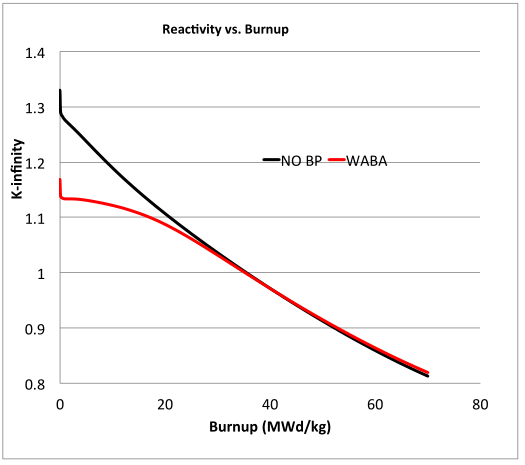
\includegraphics[width=0.5\textwidth]{images/dfs/rho-vs-BU.png}
  \caption{Reactivity vs. BU} \label{rho-vs-BU}
\end{figure}

\topic{Actinide Chain Balance Equation}

Normally we would model around 400 actinides; for this class, we only
discuss 22 of them that occupy the high-end of actinides (with large
N, large Z).


What happens during actinide chain construction?

\begin{enumerate}
\item FP absorbe neutrons and reduce reactivitiy of the fuel
  significantly, often 10-20\%;

\item Fission cross section: isotopes have threshold energies,
  producing step-shape near higher energies (around 10
  MeV)\footnote{Both even and odd isotopes have threshold energies,
    but odd isotopes have higher resonance fission cross section,
    hence even isotopes' threshold energy behavior is more
    pronoud.}. Remember Pu is very fissile material. Am242 is a funny
  one -- although it's an even isotope, its fission cross section is
  large.

\item Simple actinide nuclide transmutation model as in
  Figure~\ref{actinide-model}: red arrows designate the actinide
  chains we model (chains end at isotopes that decay quickly compared
  with the phenomena we are trying to model); blue arrows designate
  beta decay.
\begin{figure}[h]
  \centering
  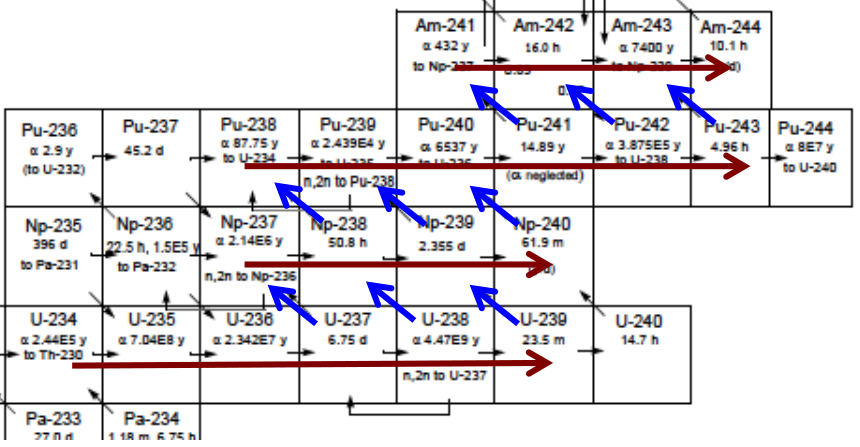
\includegraphics[width=0.7\textwidth]{images/dfs/actinide-model.png}
  \caption{Simple Actinide Nuclide Transmutation Model} \label{actinide-model}
\end{figure}

\item The higher you go up the chain (e.g., into the MA region), the
  worse the absorption would be.

\item Branching ratio is a function of energy. Example: \ce{^{241}Am}
  can produce \ce{^{242}Am} with a half-life of 16 hrs, and the
  meta-stable \ce{^{242m}Am} with a half-life of 141
  years. \ce{^{242}Am}'s thermal branching ratio is about 10\% that of
  \ce{^{242m}Am}.
\end{enumerate}

\begin{figure}[ht]
  \centering
  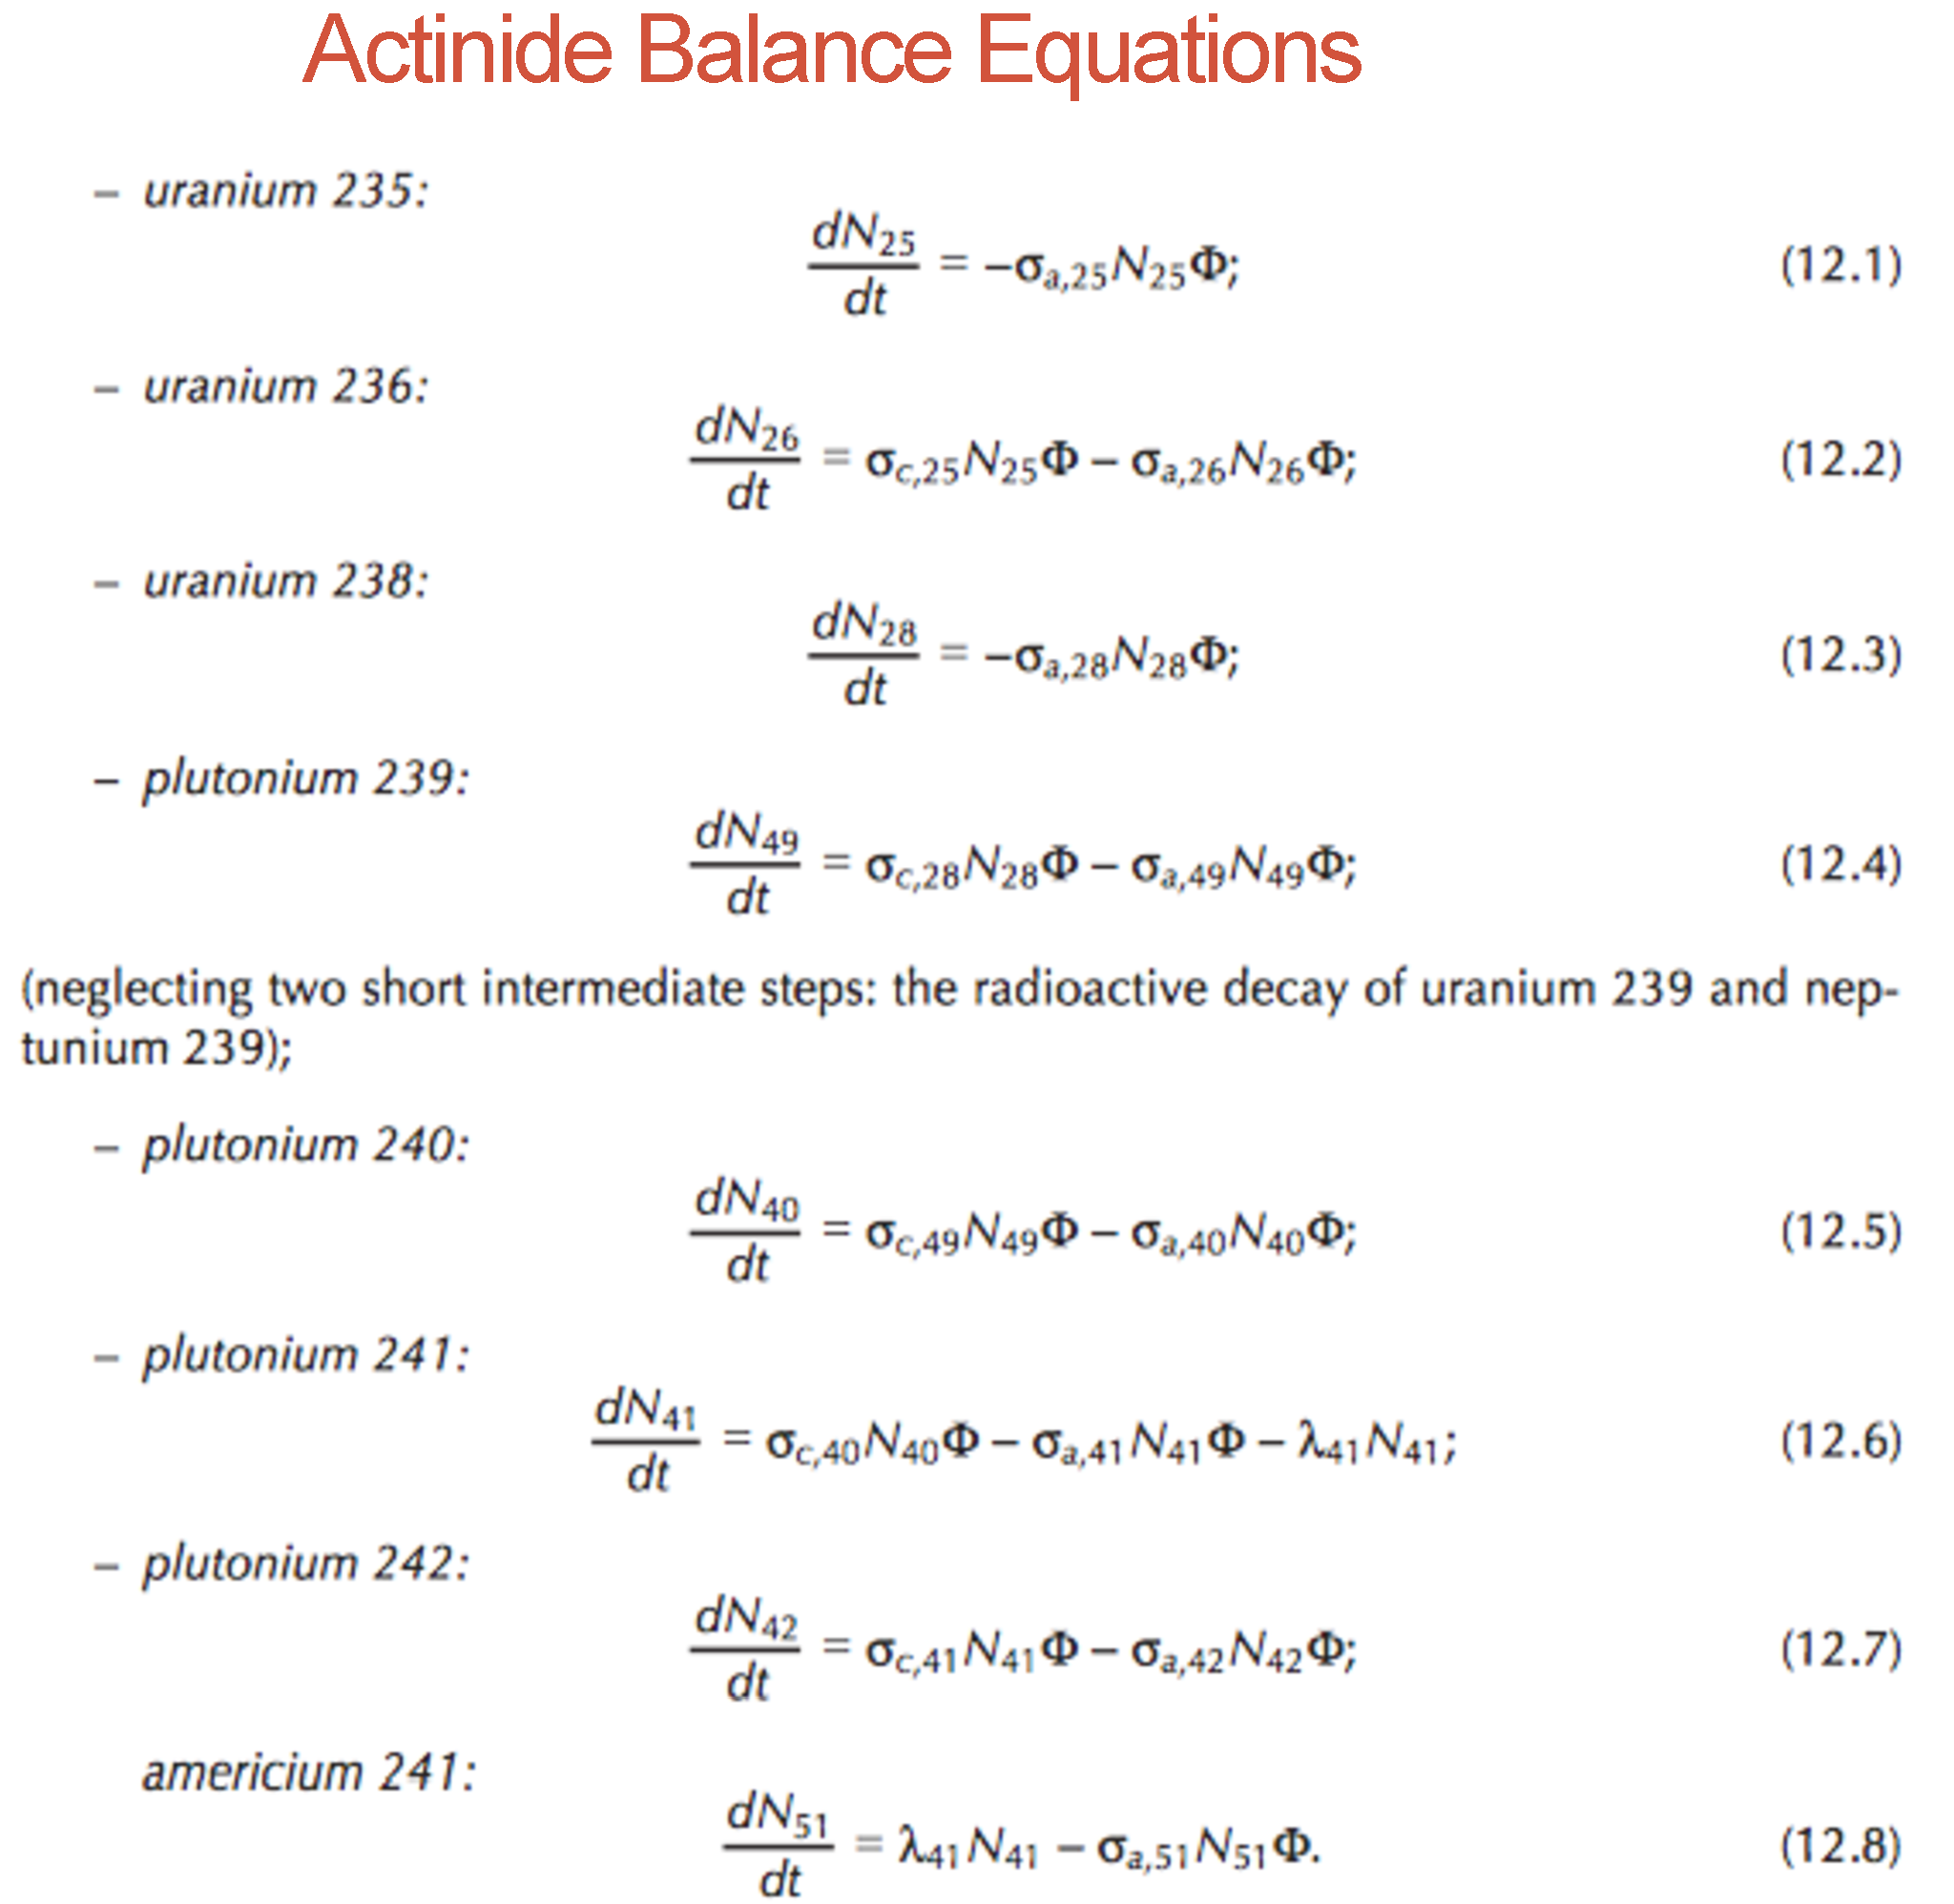
\includegraphics[width=5in]{images/dfs/actinide-balance.png}
  \caption{Actinide Balance Equations}
\end{figure}

\clearpage
\topic{Actinide Chain Matrix System} 

Compare fission product matrix form vs. actinides matrix formin
Fig.~\ref{fp-an-matrix-form}:

\begin{itemize}
\item Actinides matrix form has no fission yield term so the solution
  is just $[N(t_n)] = e^{-[A] \Delta t_n} [N(t_{n-1})]$ ;

\item FP matrix is decoupled; actinide matrix is not. 
\end{itemize}
\begin{figure}[ht]
  \centering
  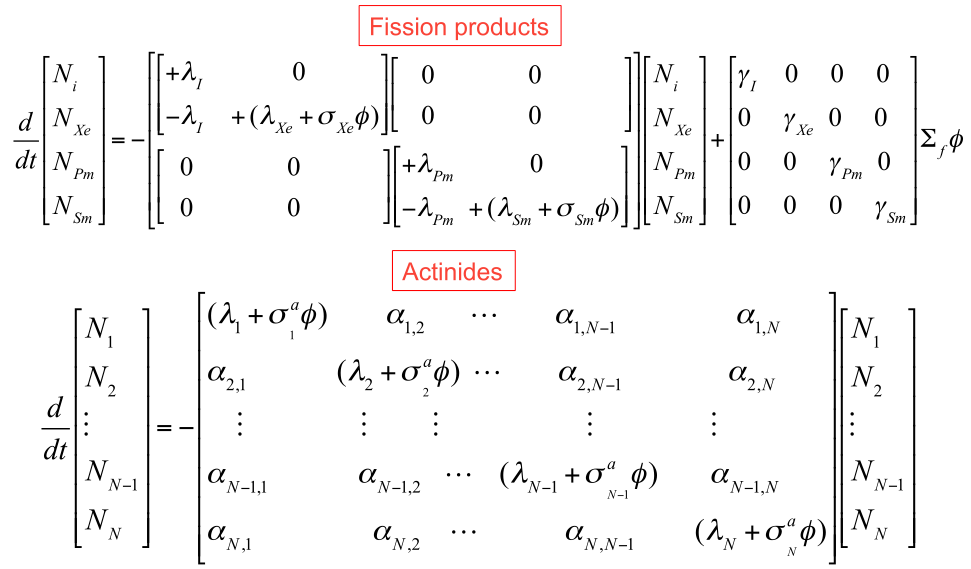
\includegraphics[width=5in]{images/dfs/fp-an-matrix-form.png}
  \caption{Nuclide Depletion Equations vs. Actinide in Matrix
    Form} \label{fp-an-matrix-form}
\end{figure}

More specifically, we focus on the actinides matrix which is
illustrated in both Fig.~\ref{nuclide-depletion-matrix} and
Fig.~\ref{actinide-block}.

\begin{figure}[ht]
  \centering
  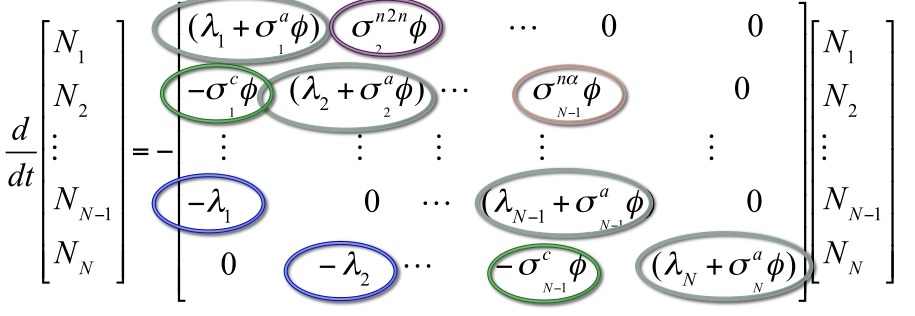
\includegraphics[width=5in]{images/dfs/nuclide-depletion-matrix-form.png}
  \caption{Nuclide Depletion Equations vs. Actinide in Matrix
    Form} \label{nuclide-depletion-matrix}
    \end{figure}
There are 4 blocks for the 4 species as in Fig.~\ref{actinide-block}. 
\begin{figure}[ht]
  \centering
  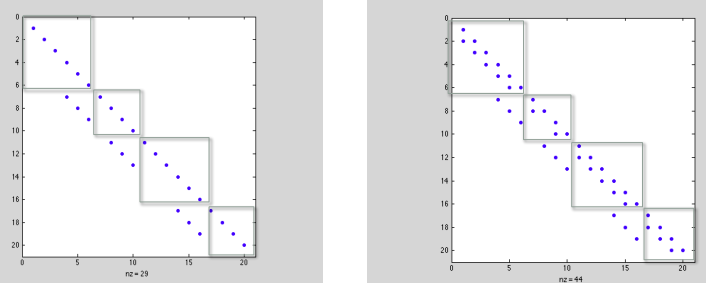
\includegraphics[width=5in]{images/dfs/actinide-block.png}
  \caption{Matrix Shape for Actinide Depletion
    Equations} \label{actinide-block}
    \end{figure}
\begin{itemize}
\item The decay terms sit outside of the blocks; they couple the blocks.
\item The capture terms are one line off the diagonal term (NP238
  decays so quickly that its capture cross section is zero and is not
  shown through the spy function in Matlab);
\item We don't have above the diagonal term because we ignore the
  $n2n$ reaction and the $n \alpha$ reaction. The reason we ignore
  them is that having a sub-diagonal matrix we can invert
  analytically; whereas having a full matrix is a lot harder to
  invert. Another simplification we made is to ignore all meta-stable
  states and only have the ground states, hence ignoring branching.
\end{itemize}

One side-note here is that Bateman equations can be very stiff. For a
system of differential equation 

\eqn{ \left[ \begin{array}{c} N_1' \\ N_2' \\ N_3' \end{array} \right]
  = \left( \begin{array}{ccc} -\lambda_1 & 0 & 0 \\ \lambda_1^1 & -
    \lambda_2 & 0 \\ \lambda_1^2 & \lambda_2 & 0 \\ \end{array}
  \right) \left[ \begin{array}{c} N_1 \\ N_2 \\ N_3 \end{array}
    \right] }

whose solution is expressed as $[N] = [V] [\Lambda] [V]^{-1} [N_0]$ where 

\eqn{ [\Lambda] &= \mathrm{Diag} [e^{-\lambda_1 t}, e^{-\lambda_2 t},
    1] & [V] &= \left( \begin{array}{ccc} 1 & 0 & 0
    \\ \frac{\lambda_1^1}{\lambda_2 - \lambda_1} & 1 & 0
    \\ \frac{\lambda_1^2 - \lambda_2}{\lambda_2 - \lambda_1} & - 1 & 1
    \\ \end{array} \right) } 

So if $\lambda_1 = \lambda_2$ (which is possible when absorption terms
are present), \hi{numerical instability} could happen depends on the
flux level!

\clearpage
\topic{Actinide Chain Solution}
\begin{figure}
  \centering
  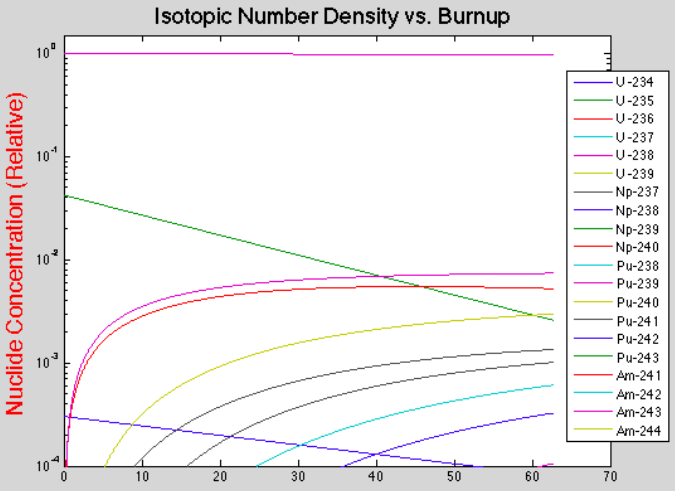
\includegraphics[width=0.8\textwidth]{images/dfs/actinide-vs-BU.png}
  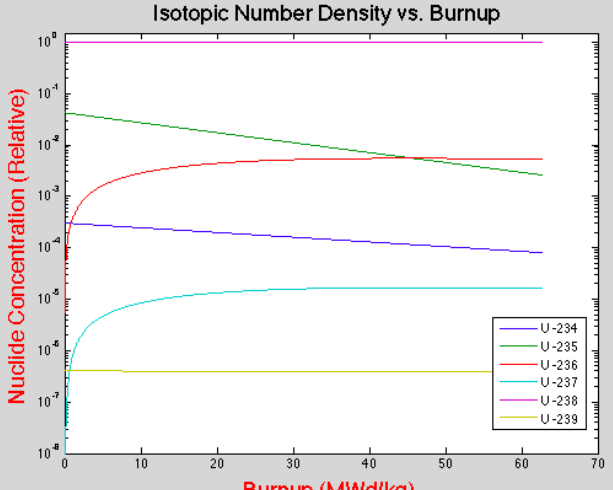
\includegraphics[width=0.45\textwidth]{images/dfs/actinide-vs-BU-1.png}
  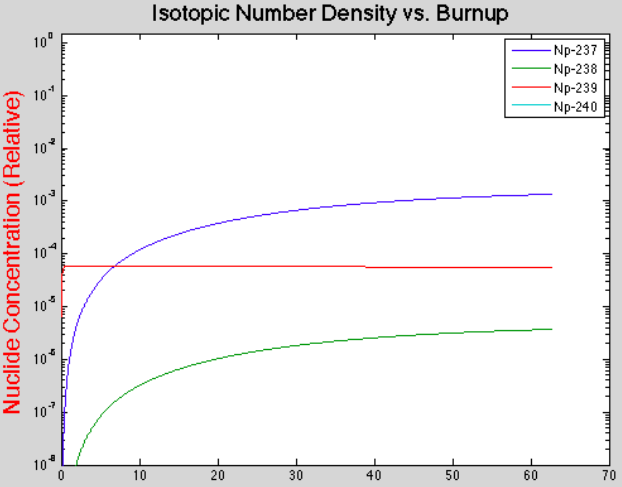
\includegraphics[width=0.45\textwidth]{images/dfs/actinide-vs-BU-2.png}
  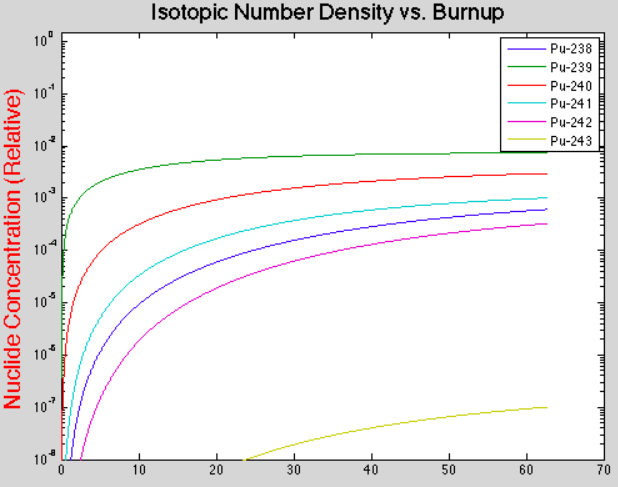
\includegraphics[width=0.45\textwidth]{images/dfs/actinide-vs-BU-3.png}
  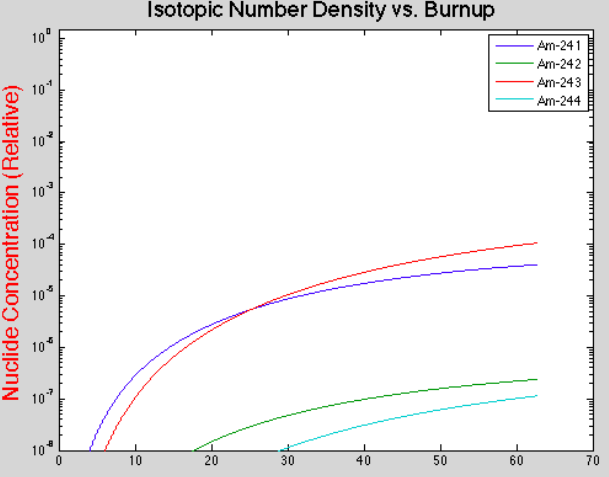
\includegraphics[width=0.45\textwidth]{images/dfs/actinide-vs-BU-4.png}
  \caption{Actinide Concentrations vs. BU} \label{actinide-vs-BU}
\end{figure}

Interpretation of Fig.~\ref{actinide-vs-BU}: 
\begin{enumerate}
\item U238 barely changes; there are a lot of it, and it probably
  decreases by 1\%; often time the nuclear concentration is plotted
  with respect to initial heavy metal inventory, that is, U238
  concentration.
\item U234, U235 does not have production, hence it decreases. 
\item U236 is produced as we burnup U235; U236 has almost no
  destruction rates;
\item U237 is produced as we burnup 
\item U239 is a constant because its capture from U238 is constant,
  and U239 decays so quickly (23 mins) that it's at equilibrium the
  whole time.
\item (remember) Np has a half-life of 2 and 2.5 days; Np's cancels
  out Am etc, and they have the same half-life, so people use to
  ignore them.
\item Production with Pu; 
\item Am244: takes a certain burnup to come up. Even though Am is a
  small concentration, we still care about them.
\end{enumerate}
\begin{figure}
  \centering
  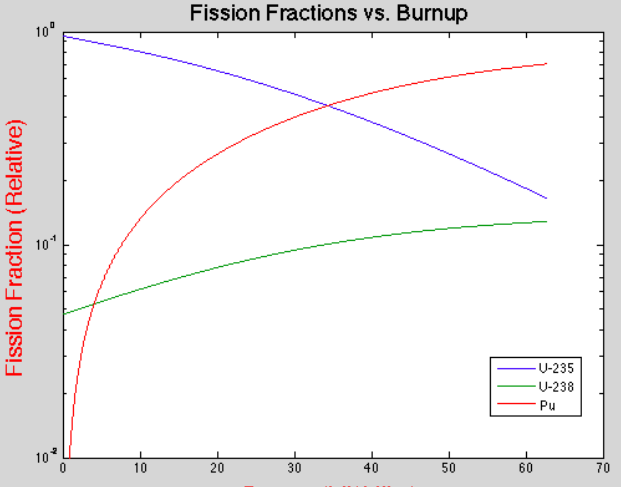
\includegraphics[width=0.7\textwidth]{images/dfs/ff-vs-BU.png}
  \caption{Fission Fractions by Nuclide vs. BU} \label{ff-vs-BU}
\end{figure}
Fig.~\ref{ff-vs-BU} shows that about 40-50\% of power would be
produced from Pu instead of U by the time we shut down the reactor.

\clearpage
\topic{Burnup: Why we use it and units}
\begin{figure}[h]
  \centering
  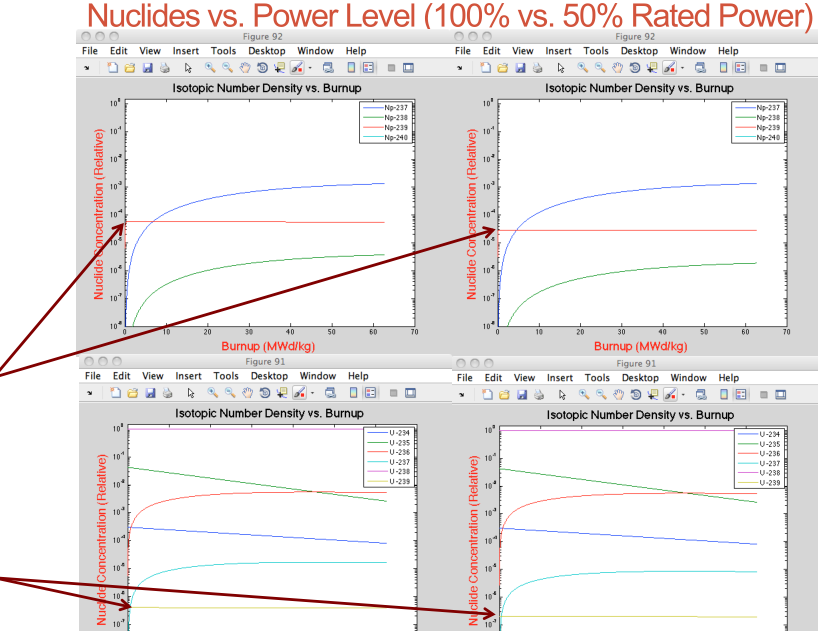
\includegraphics[width=0.8\textwidth]{images/dfs/nuclide-vs-power.png}  
  \caption{Isotropic Number Density vs. BU} \label{n-vs-BU} 
\end{figure}
Fig.~\ref{n-vs-BU} shows that power level does not affect number
density vs. BU plot. BU is a better gage of depletion effect than
time.

\begin{enumerate}
\item FIFA = fission per initial fissile atoms;
\item FIMA = fission per initial (heavy) metal atoms;
\item Atom percent (A\%) = FIMA * 100;
\item Burnup: GWd/T = MWd/kg = thermal power per weight of heavy metal. 
  \begin{itemize}
    \item Advantages: we know the reactor power and initial fuel
      loading (almost).
    \item Disadvantages: `energy released' is not a very clean term;
      we don't really care about neutrino energy, gamma energy
      released from capture of neutrons; energy deposited in fuel
      assembly B from fissions in assembly A etc. In LWR, it is a good
      approximation to assume that energy is depositied locally where
      the fission happens; in MITR it is a bad approximation, fission
      product energy (deposite locally), gamma heat energy (not
      necessarily deposited locally), etc.
  \end{itemize}
\item EFPHs = Effective Full Power Hours; EFPD = Effective Full Power Days. 
\end{enumerate}

\clearpage
\topic{History Effects}
\begin{enumerate}
\item Overall, we use WABA (Wet Annular Burnable Absorber), IFBA
  (Integral Fuel Burnable Absorber) and Gd (mixed with fuel) to
  control reactivity.
  \begin{figure}
    \centering
    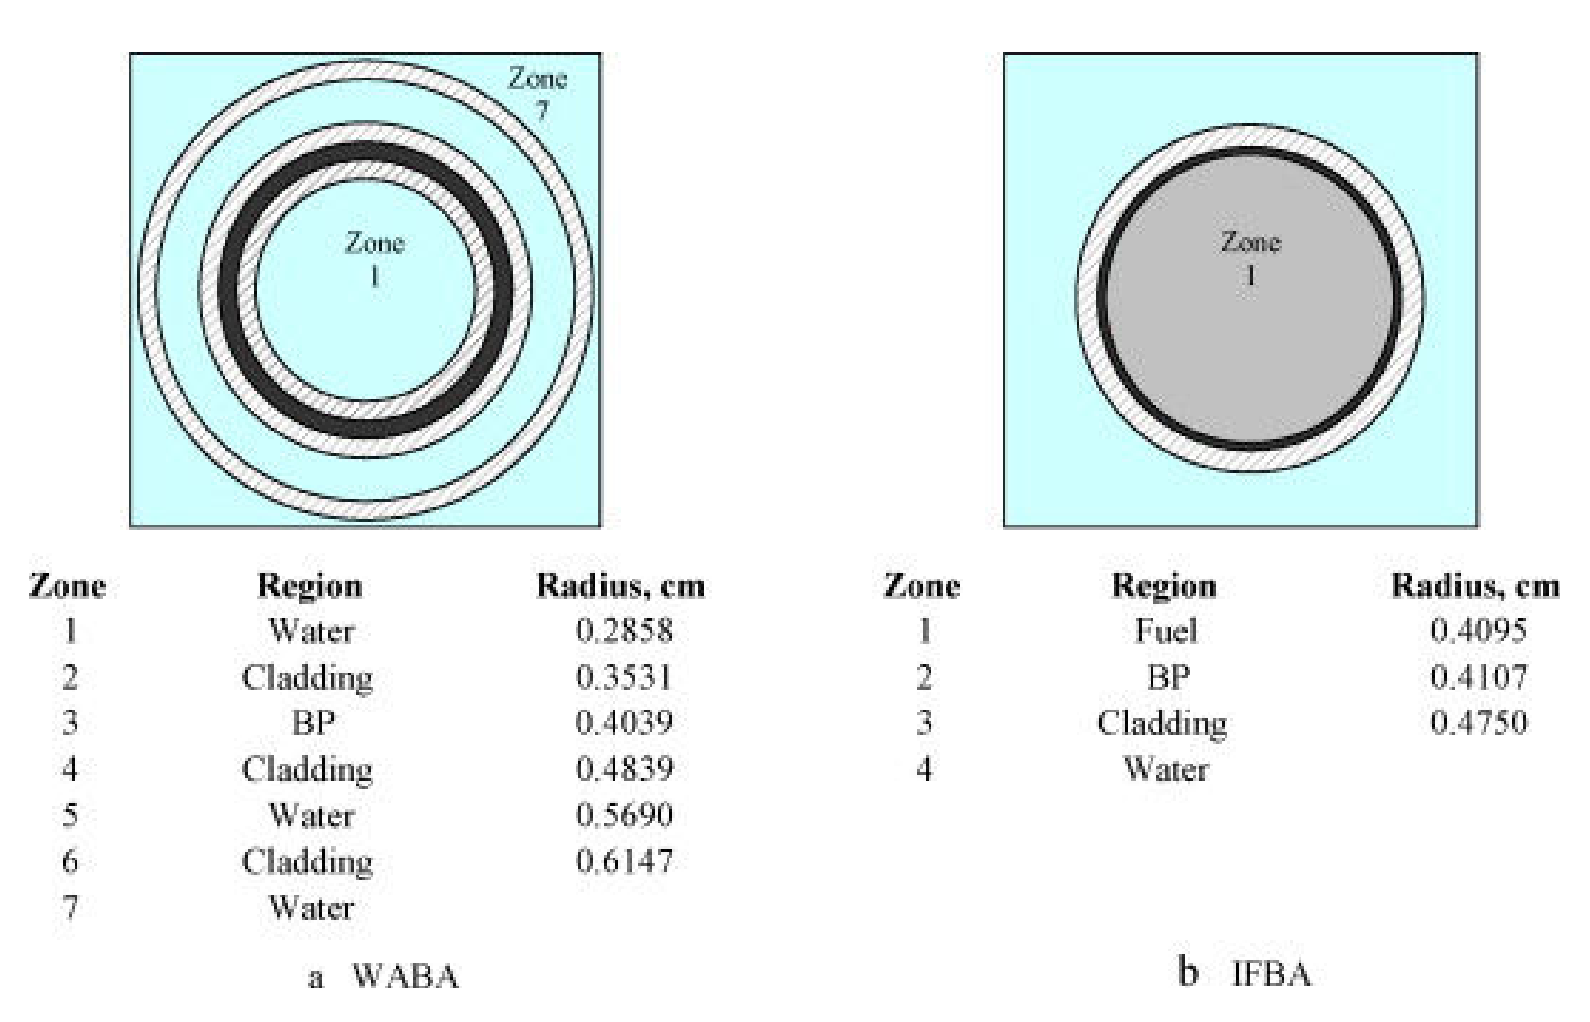
\includegraphics[width=4in]{images/dfs/WABA-IFBA.png}
    \caption{Composition of WABA and IFBA} 
  \end{figure}

\item Burnable Poisons History Effect (Fig.~\ref{BP-history-effect}):
  hardern the spectrum, because it pushes some water away. It is a
  history effect: you place BP at BOL and take it out later to achieve
  flat power through time. \hi{The BP effect is about 250 pcm}.
  \begin{figure}
    \centering
    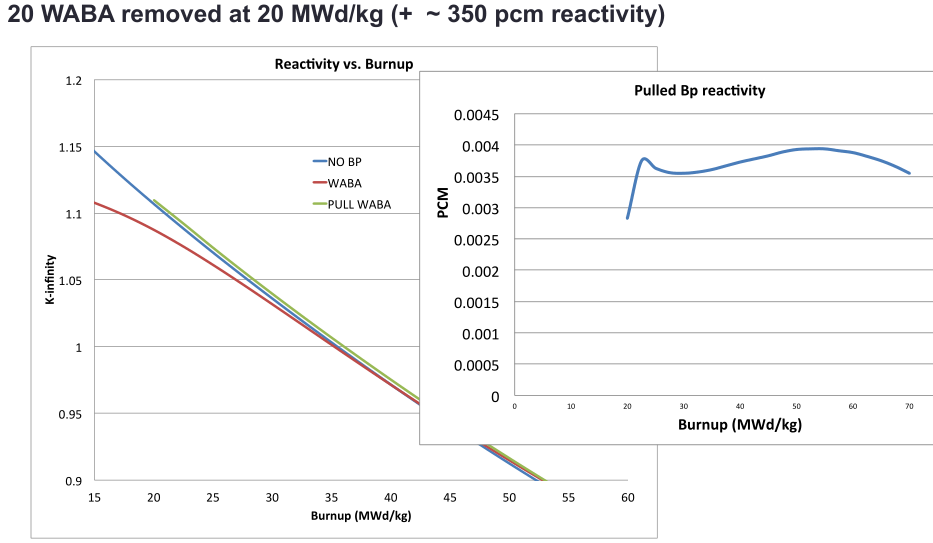
\includegraphics[width=5in]{images/dfs/BP-history-effect.png}
    \caption{Removable Burnable Poisons: History Effects}  \label{BP-history-effect}
  \end{figure}


\item Fuel Temperature Depletion History Effects (Fig.~\ref{dhe}):
  initially, the instantenous temperature effect is almost independent
  of depletion; as the burnup increases, something happens. The moral
  of the story is, we not only need to know the burnup but also the
  temperature.
  \begin{figure}
    \centering
    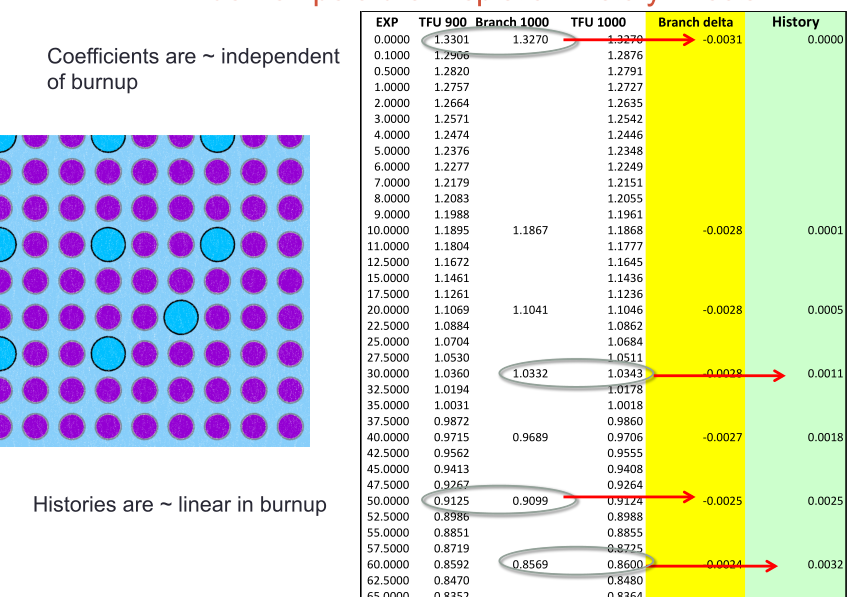
\includegraphics[width=5in]{images/dfs/depletion-history-effect.png}
    \caption{Fuel Temperature: Depletion History Effects}  \label{dhe}
  \end{figure}

\item Gadolinium burnable absorber (Fig.~\ref{Gd-BP}): 
  \begin{itemize}
  \item Gadolinium has a huge thermal absorption cross section. It is
    almost as high as Zn, but we cannot use Zinon because it would
    decay;
  \item What we do with Gadolinium is to replace part of the fuel with
    Gd and reactivity would be flatter with respect to time.
  \item Gad depletes/burns in layers around the fuel pin from outside
    to inside. ]
  \item Hold-down is the difference between the reactivity at the BOL
    with and without the reactivity control mechanism.
  \item Gad residual: there is a little bit loss of reactivity due to Gad. 
  \end{itemize}
  \begin{figure}
    \centering
    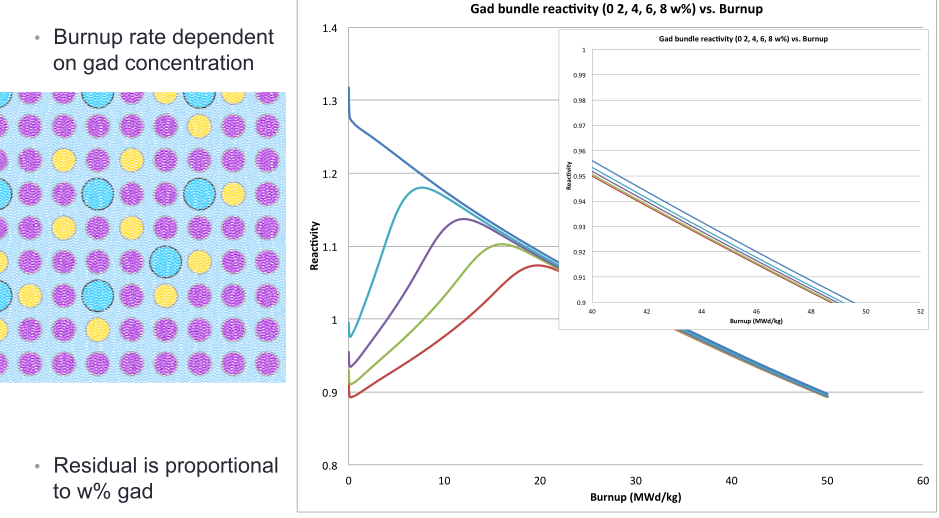
\includegraphics[width=5in]{images/dfs/Gd-BP.png}
    \caption{Gd Burnable Poisons}  \label{Gd-BP}
  \end{figure}
\end{enumerate}



\clearpage
\topic{Numerous Subtle Effects}
\begin{enumerate}
 \item We didn't really cover the Thorium/U233 Chain in Kord's class. 
   \begin{itemize}
   \item The chain for Th is very complicated; there are n2n reactions
     at all different levels; there are multiple ways to get U232;
   \item some of these isotopes have very rapid alpha decays; 
   \item Pa233 has 27 day half-life; 
   \item U232 has 70 year half-life; U232's daughter product Ta208 has
     2.6 MeV gamma (which is the hardest gamma known).
   \end{itemize}
   \begin{figure}[h]
     \centering
     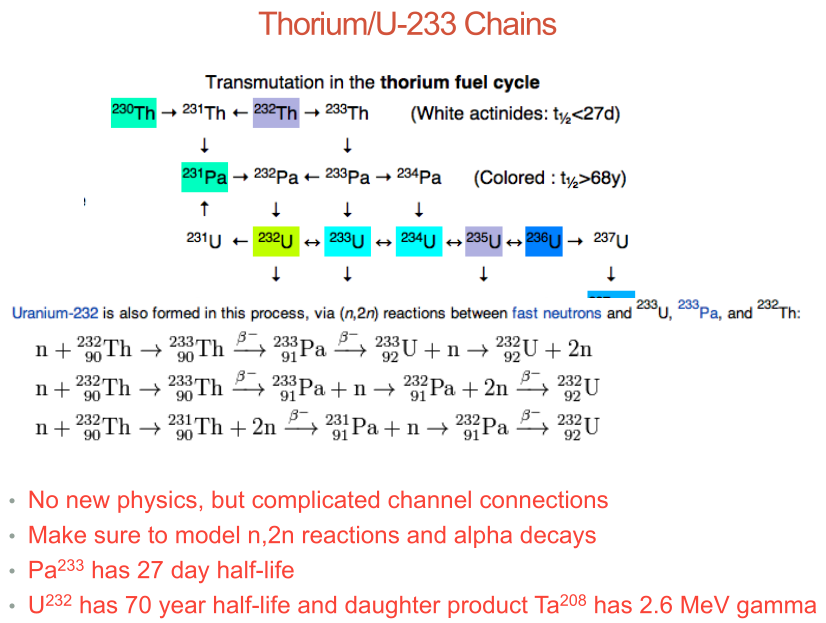
\includegraphics[width=4in]{images/dfs/Th-U-chains.png}
     \caption{U233/Th Chains} 
   \end{figure}


\item Coverage of Th/U233 comparison from Ben's class (11/29). 

  \begin{tabular}{ccc}
    \begin{minipage}[b]{0.3\linewidth}
      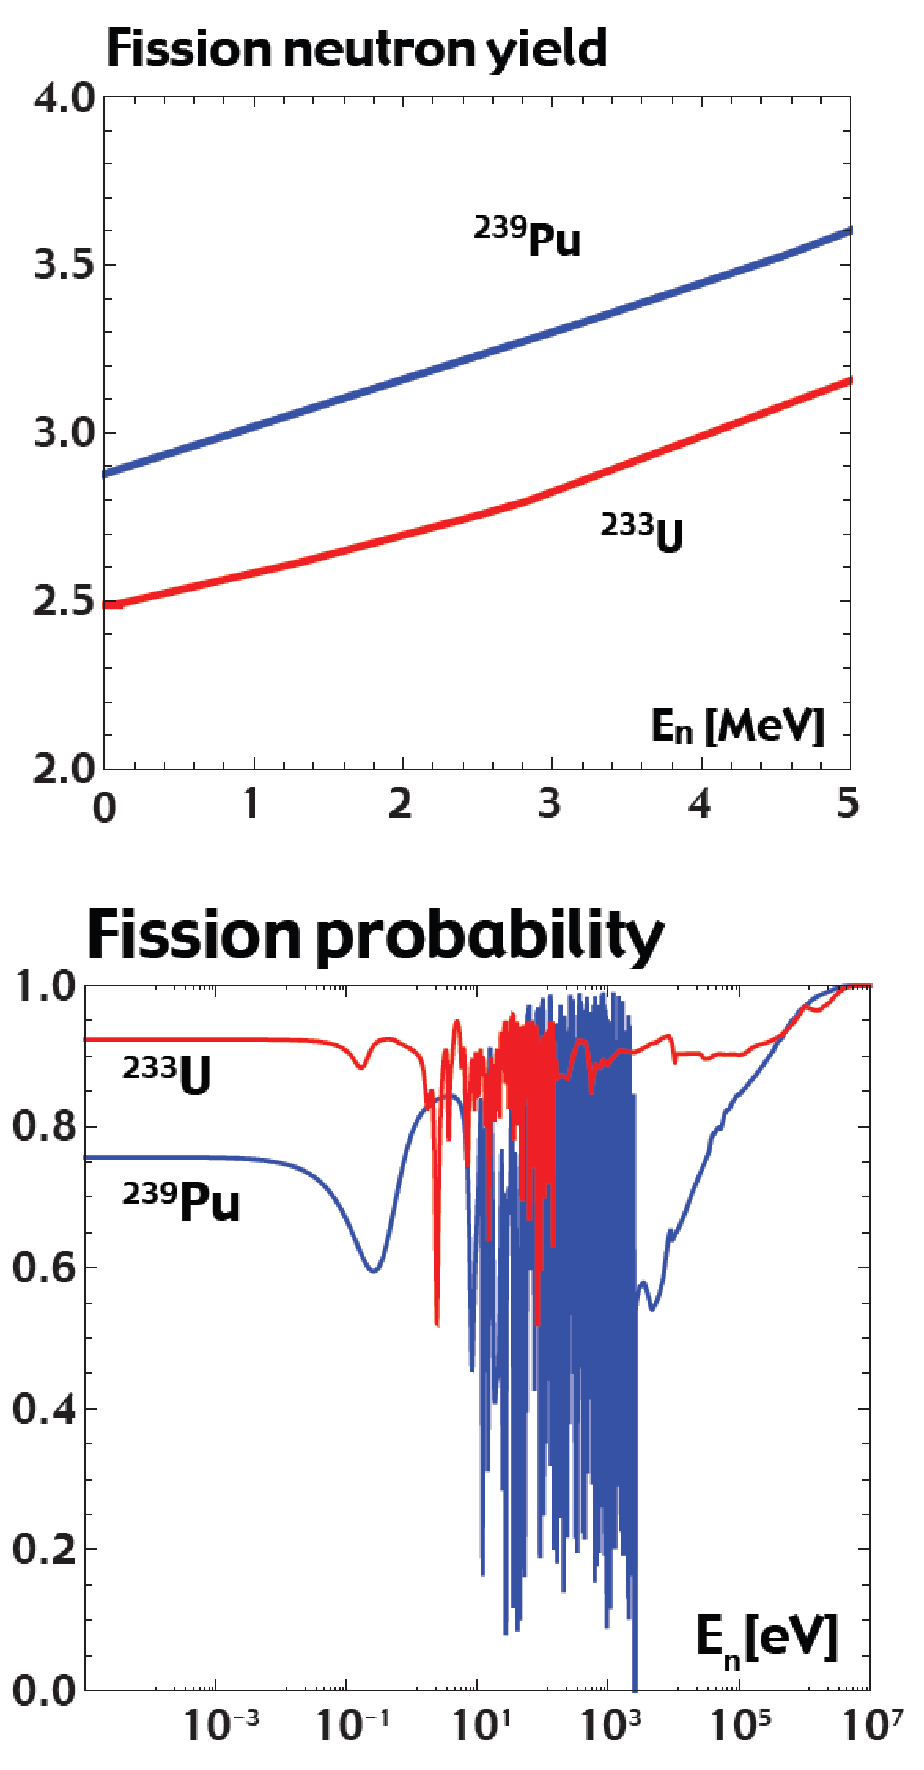
\includegraphics[width=\textwidth]{images/dfs/U-vs-Th.png}
    \end{minipage}
    &
    \begin{minipage}[b]{0.3\linewidth}
      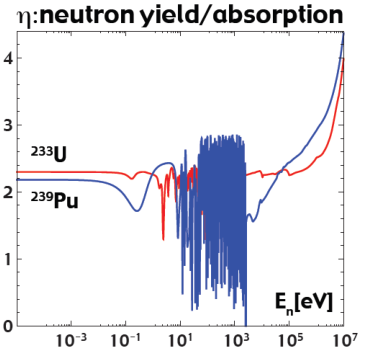
\includegraphics[width=\textwidth]{images/dfs/U-vs-Th-2.png}
    \end{minipage}
    &
    \begin{minipage}[b]{0.38\linewidth}
      \begin{itemize}
      \item Neutron yield increases with incoming neutron energy, and
        Pu239 produces almost 0.5 more neutron per fission.
      \item But fission probability once captures in larger in U233
        except at high energy.
      \item Combining the two graphs yields: $\eta = \frac{\nu
        \sigma_f}{\sigma_f + \sigma_c}$. Thus Th cycle is preferable
        for breeding in thermal systems.
      \end{itemize}
    \end{minipage}
  \end{tabular}
      
\item Th cycle advantages: 
\begin{enumerate}
\item Abundancy is 4x that of U. 
\item Less waste: we start further bottom left from the chain, and Th
  cycle would generate less MA waste.
\item U-233 critical mass is smaller than U-235 and not diluted by U-238. 
\item U-232 emits high energy gamma. 
\item Difficult reprocessing. 
\end{enumerate}
Companies that considers Th cycle: Thorium Power Inc which is a
subsidiary of Lightbridge Corp.
\begin{table}
  \centering
  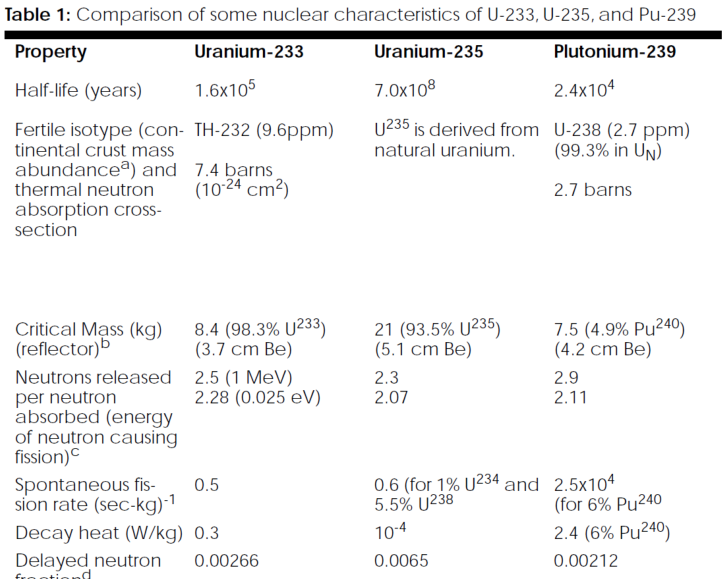
\includegraphics[width=5in]{images/dfs/fuel-type.png}
  \caption{Nuclear Fuel Characteristics} 
\end{table}

\item Where do reaction rates come from? 
  \begin{itemize}
  \item ORIGEN uses point depletion, 
  \item Fuel pin radial shape: the outter region almost have 2 times
    the flux compared with the inner ones.
  \end{itemize}

\item Benchmark: 
  \begin{itemize}
  \item data set is the single most important things in determine the
    accuracy of your codes.
  \item U235 has a pretty large error, but we don't care because there
    is so little of it;
  \item Accuracy tends to decrease the further up the decay chains. 
  \item Measurements also have an intrinsic uncertainty; do not rely
    on single measurement campaigns; systematic errors in measurements
    are common.
  \item In performing `actinide burner' analysis, when we place the
    actinide at the end of one analysis into another one, the error
    builds up.
  \end{itemize}
\end{enumerate} 



\clearpage
\topic{Spent Fuel and Recycling} 

\subtopic{Neutronic Consideration}

The following spent fuel neutronics was given by Prof. Forget on
11/29/12 for 22.211.

\begin{enumerate}

\item Spent fuel: 15\% of U-235 transmuted to U-236 and Np-237. 3.5\%
  of U-238 transmuted to Pu-239. That is, \hi{60\% fissioned} and the
  rest remains Pu-239 and higher actinides.

\item The majority of the spent fuel is U238 which is not real waste;
  the U and Pu in the spent fuel is sent back to the core. The real
  waste is limited to MA and is vitrified in a borosilicate glass
  form.

\item MOX recycling: spent fuel contains enough fissile Pu to be
  recycled in a LWR. \ce{Pu O_2} is mixed with depleted U (enrichment
  varies between 5 to 8\% Pu). Pu recycling reduces amount of waste by
  30 \% (reduce total TRU by 20\%), but has minimal impact on
  radiotoxicity. MOX core loading is currently being done in France,
  Germany, Belgium, Switzerland and Japan. Current PWR are limited to
  30\% loading of MOX assemblies b/c:
  \begin{itemize}
    \item Pu reduces the delayed neutron fraction. 
    \item MOX fuel has a harder spectrum thus reducing the efficiency
      of the control rods and soluble boron.
    \item Create pin peaking at the edge of MOX and UOX assemblies.
  \end{itemize}
  Newly designed PWRs would be able to accommodate full core MOX
  assemblies by:
  \begin{itemize}
    \item $\up$ number of control rods. 
    \item $\up$ boron enrichment. 
    \item $\up$ moderator to fuel ratio. 
  \end{itemize}

\item A higher Pu enrichment is typically required compare to U for
  two reasons: a) only 60\% Pu is fissile \ce{^{239}Pu}, the rest of
  them are parisitic; b) Pu has a higher absorption rates.
  \begin{figure}[h]
    \centering
    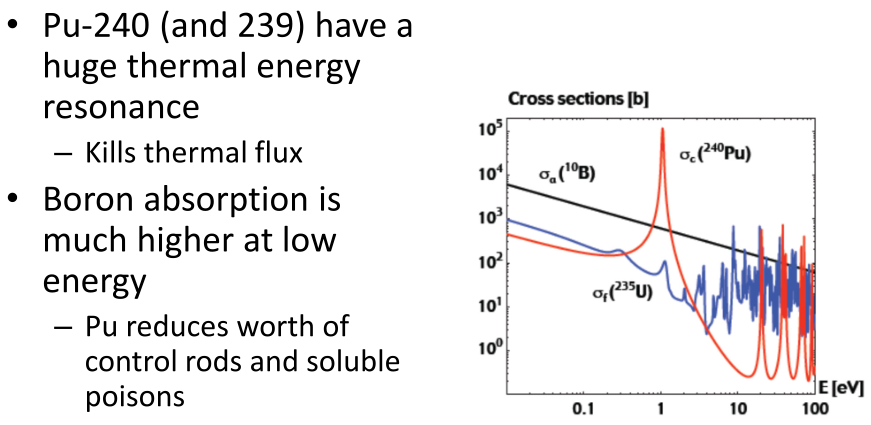
\includegraphics[width=4in]{images/dfs/Pu-fuel.png}
  \end{figure}


\item Multi-recycling: we cannot recycle too many times. Reason: after
  1st cycle the fissile content is 64.8\%, after 2nd cycle fissile is
  only 51.1\% and requires a higher Pu enrichment; and if Pu
  enrichment is pass xxx, then the void coefficient would become
  positive.
  \begin{figure}[h]
    \centering
    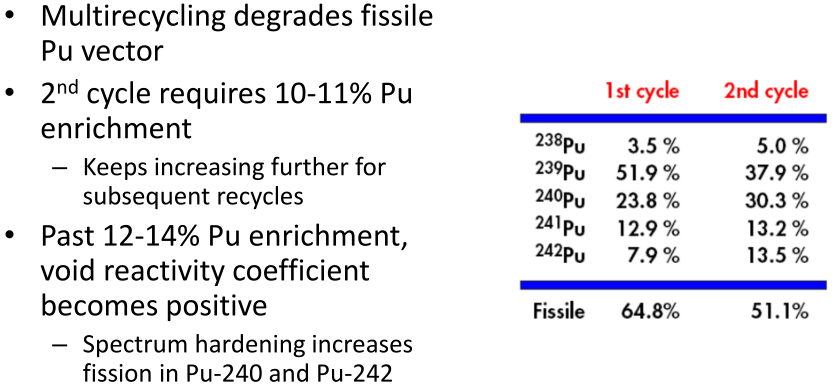
\includegraphics[width=4in]{images/dfs/multirecycling.png}
  \end{figure}

\item DUPIC cycle (used in CANDU): it is an entirely mechanical
  process during which we grind up everything, the gas comes out, and
  re-construct the grinds into fuel which contains about 0.8\% U235
  and 0.8\% Pu239, which is about twice the excess reactivity of
  natural uranium and is more than enough for a CANDU.

\item Fast reactor transmutation: at high energy, all MA are fissionable
  (also high absorption cross section which is why we don't expect to
  get energy from MA), so we can transmutate MA.

\item Safety concerns: See Fig.~\ref{safety-concern}.
 
  \begin{figure}[h]
    \centering
    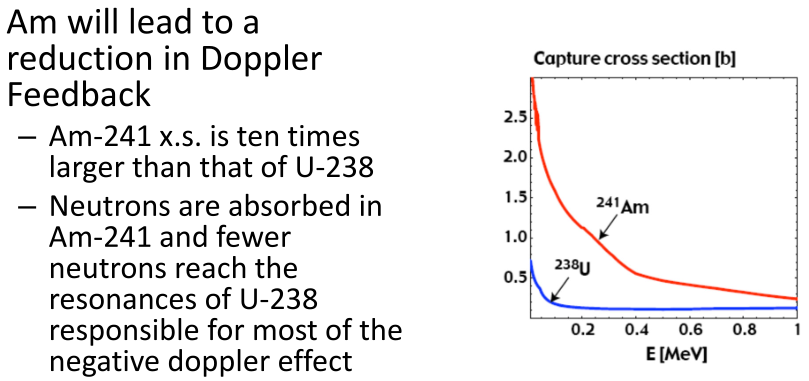
\includegraphics[width=0.45\textwidth]{images/dfs/safety-Doppler.png}
    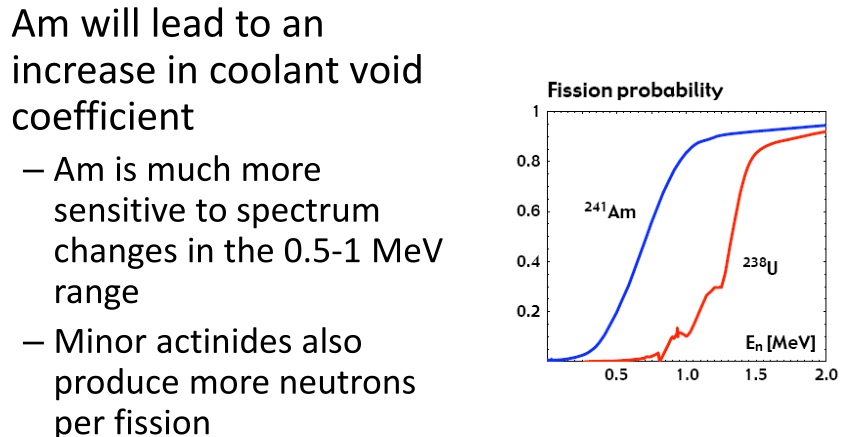
\includegraphics[width=0.45\textwidth]{images/dfs/safety-void.png}
    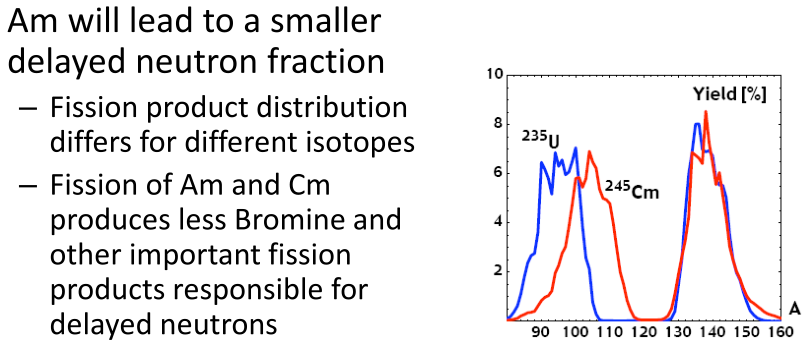
\includegraphics[width=3.2in]{images/dfs/safety-delayed-neutrons.png}
    \caption{Safety Concerns} \label{safety-concern}
  \end{figure}
\end{enumerate}


\subtopic{Spent Fuel Storage}

There are a couple of places that we store spent fuel

\begin{enumerate}

\item Spent fuel pool (SFP): 
  \begin{enumerate}
    \item Typically the three units in the same site share the same
      spent fuel pool.
      
    \item Requirement: $\keff < 0.95$. 

    \item SFP design simulation: it is common to use MCNP to calculate
      the inter-assembly spacing to keep $\keff$ under the
      limit. US-APWR licensing assumes all fresh fuel in SFP. SFP
      absorber panels were placed inside to reduce the inter-assembly
      spacing. The absorber panels are made of B-10 in the form of
      \ce{B_4C} in a metal matrix or a polymer matrix Boraflex
      (trademark of BISCO). Boraflex is great, except it degenerates
      with gamma radiation which was not known at the time of
      construction.

    \item Other licensing simulation: calculate dilution time needed
      to reach 200ppm. That is, assuming a 200ppm perturbation, how
      much dilution do we need to keep it subcritical?

    \item Make most conservative assumptions possible: water density
      at its lowest, water temperature at its highest, worst axial
      distribution etc.

    \item SFP loading curves are developed where the y-axis is Burnup,
      x-axis is initial enrichment, and lines were drawn to illustrate
      limitations. 
  \end{enumerate}

\item Interim Storage: CLAB (Central Interim Storage Facility for
  Spent Fuel) is an interim storage facility for all spent fuel from
  Swedish nuclear reactors. It was opened in 1950 and was expanded in
  the 2000s to its current capacity. A Swedish reactor generates
  between 15 to 25 tonnes per year. It has also been used for
  performing calorimeter measurements of full-length spent fuel
  assemblies.

\item On-site dry cast storage. These are dry casks built
  on-site. Under the current consideration, all sites are going to get
  dry cast storage eventually. It consists of steel canisters (one
  canister holds 36 assemblies), storage casts, and transport
  casts. Loading 36 assemblies into a canister takes about 1.5
  days. Each fuel transport operation (placing canister in cast, two
  welded steel lids, take out water and pump in He) takes about 8 days
  to complete. At Yankee Rowe, the inner cast is a transport cast that
  can be taken out and transport to a permanent site later on.
\end{enumerate}



\clearpage
\topic{Relate Neutronics and TH}
This section was given by Prof. Forget on 12/04/12 and 12/06/12. 
\begin{enumerate}
\item FP deposit energy locally, and fuel expands due to temperature
  changes. Because the temperature increase on the inside is larger
  than the outside, pellets are fabricated with a slightly shorter
  height on the inside as in Fig.~\ref{fuel_pellets}
\begin{figure}[ht]
  \centering
  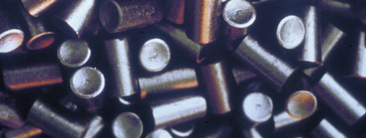
\includegraphics[width=4in]{images/dfs/fuel_pellets.png}
  \caption{Fuel Pellets Shapes} \label{fuel_pellets}
\end{figure}


\item \ce{UO_2} is used in LWRs regardless of its low heat transfer
  property because it does not interact with water
  violently. \ce{UO_2} has a relatively low thermal expand, so the gap
  between the fuel and the clad can be relatively small.

\item Fast reactors use metallic fuel because a) better heat transfer,
  b) coolant is not water so no worry for chemical reaction, c)
  metallic fuel thermal expansion is large, which replaces Doppler
  effect(recall Doppler is due to U238 -- ). Also because metallic
  fuel expands more, we build fuel pellets with more porosity to limit
  the amount of volume expansion.

\item Grid straps: egg crates to place pins in them. Pin starts
  vibrating and may cause fuel failure.

\item To flattern power peaking: 
  \begin{enumerate}
  \item Core loading. 
  \item Poisons: WABA, IFBA \ce{Zr B_2}, Gd and other Lanthanum. 
  \item Control rod sequence. 
  \item Reflector. 
  \item Core enrichment. 
  \item Flow orificing: change flow pattern at different
    assemblies. It is not done in LWRs that often, more common in SFRs
    to control temperature and flux spectrum.
  \end{enumerate}

\item Thermal transients in fuel: \eqn{ M_F C_{p,f} \frac{\dT_f}{\dt}
  = P(t) - \frac{1}{R_f} (T_f(t) - T_c(t)) } where $R_f$ captures all
  the thermal resistance. Assume steady state, then \eqn{ P(t) =
    \frac{1}{R_f} (T_f(t) - T_c(t)) } If we assume a fast transient
  with no cooling ($R_f \to \infty$), then we get adiabatic heat rate:
  \eqn{ M_f C_{p,f} \frac{\dT_f}{\dt} = P(t) }


\item Thermal transients in coolant: 

\eqn{ M_C C_{p_C} \frac{\dT_c}{\dt} = \frac{1}{R_f} (T_f(t) - T_c(t))
  - 2 \dot{m}_c C_{p_c} (T_c(t) - T_i) }

where $\dot{m}$= mass flow of coolant, and the factor of $2$ is there
because the $T_c(t)$ in the equation is assumed to be the average.
  \begin{itemize}
    \item Steady state: $\displaystyle 2 \dot{m} C_{P_c} (T_c - T_i) =
      \frac{1}{R_f} (T_f - T_c) = P$. That is, reactor power is
      determined from flow and temperature measurements.
  \end{itemize}


\item We can relate the above two equations with the PKE using
  $P(t)$. That is, how do we relate temperature change to reactivity
  change.
 
  \begin{enumerate}

    \item Set-up: consider $\displaystyle \rho = \frac{k-1}{k}, \drho
      = \frac{\dk}{k^2}$. If we assume $k \approx 1$, then
      $\displaystyle \drho = \frac{\dk}{k} = \derivative(\ln
      k)$. There is benefit in writing $k$ in log form as now we can
      separate multiplication into additions.

  \item Consider $\keff = \kinf P_{NL}$, where $P_{NL} = \frac{1}{L^2
    B_g^2}$, we can write, 

    \eqn{ \derivative (\ln k) = \derivative(\ln \kinf) +
      \derivative(\ln P_{NL}) = \frac{\dk_{\infty}}{\kinf} +
      \frac{\dP_{NL}}{P_{NL}} } We can do:
    \eqn{\frac{\dP_{NL}}{P_{NL}} = - \frac{L^2 B_g^2}{1 +L^2 B_g^2}
      \left( \frac{\derivative L^2}{L^2} + \frac{\derivative
        B_g^2}{B_g^2} \right) }

  \item Recall
 
    \eqn{ \kinf = \overbrace{\left( 1 + \frac{\nu \Sigma_{f1}}{\nu
          \Sigma_{f2}} \frac{\Sigma_{a2} + D_2 B_g^2}{\Sigma_{12}}
        \right)}^{\epsilon}
      \overbrace{\frac{\Sigma_{s12}}{\Sigma_{R1}} }^{\rho}
      \overbrace{\frac{\nu \Sigma_{f2}^F}{\Sigma_{a2}^F} }^{\eta}
      \overbrace{\frac{\Sigma_{a2}^F}{\Sigma_{a2}}}^{f} }

    \item If we characterize the temperature effect as $\kinf = f(T_m,
      T_f, T_m)$. For PWR $T_m = T_c$,
 
      \eqn{ \drho = \frac{\dk_{\infty}}{\kinf} = \frac{1}{\kinf}
        \frac{\derivative \kinf}{\dT_f} + \frac{1}{\kinf}
        \frac{\derivative \kinf}{\dT_c} }

      If we define reactor coefficient, 

      \eqn{ \alpha_x = \frac{1}{\kinf} \frac{\dk_{\infty}}{\dT_x} =
        \frac{1}{\epsilon} \frac{\derivative \epsilon}{\dT_x} +
        \frac{1}{\rho} \frac{\drho}{\dT_x} + \frac{1}{f}
        \frac{\derivative f}{\dT_x} + \frac{1}{\eta} \frac{\derivative
          \eta}{\dT_x} }
  \end{enumerate}

\item Fuel temperature feedback: Doppler (Doppler broadening of
  resonances capture of \ce{^{238}U},

      \begin{itemize}
      \item Impact $\rho$ (resonance escape probability): \eqn{ \rho
        &= \frac{\Sigma_{s12}}{\Sigma_{R1}} & T_f &\up, \Sigma_{R1}
        \up, \rho \down}
    \item Impact $\epsilon$ is negliable above resonance region. 
    \item Impact $\eta = \frac{\nu \Sigma_f^F}{\Sigma_{a2}^F}$ is very
      small because fission and absorption cross section scales with
      temperature approximately the same.
    \item Impact on $f= \frac{\Sigma_{a2}^F}{\Sigma_{a2}}$ is very
      small because absorption cross section scales with temperature
      approximately the same in fuel and outside the fuel.
    \item PWR has a $\alpha_f = -0.01$ to $-0.03$ mk/degreeC. SFR is
      about the same.
      \end{itemize}
      
    \item Moderator temperature. Consider $T_m = T_c$ for PWR, 

      \eqn{ \alpha_m = \frac{1}{\kinf} \frac{\dk_m}{\dT_m} \approx
        \frac{1}{\kinf} \frac{\dk_{\infty}}{\dN_m} \frac{\dN_m}{\dT_m}
      }

      There is no resonance effect; temperature effect is felt through
      density change.
      \begin{itemize}
      \item We define expansion coefficient (volume changes at
        constant pressure) 

        \eqn{ \beta_m &= - \frac{1}{N_m} \frac{\dN_m}{dT_m} & \alpha_m
          = - \beta_m N_m \frac{1}{\kinf} \frac{\dk_{\infty}}{\dN_m} }

      \item The expansion coefficient of sodium and salt is very
        large; it will change density, cross section, and push some
        coolant outside thus changing the moderator-to-fuel ratio.

      \item For our case, two terms depend on the fuel and do not
        change much: $\epsilon, \eta$. $\epsilon$ would go up a little
        bit, as $\Sigma_{s12} = N_m \sigma_{s12} \up$ as $N_m
        \up$. Most of the effect is felt by resonance escape
        probability $p$ and thermalization factor $f$.

      \item In the resonance escape probability $p$, $\displaystyle p
        = \frac{\Sigma_{s12}}{\Sigma_{R1}} = \frac{N_m \sigma_{H,
            s12}}{\Sigma_{R1}} \down$ as $N_m \down$. The cross
        sections are considered flat, and in the $\Sigma_{R1} =
        \Sigma_a + \Sigma_{s12}$ in which $\Sigma_a$ dominates. The
        real formulation should be,

\eqn{ p = \frac{N_m \sigma_{s12,m} + \overbrace{N_F
      \sigma_{s12,F}}^{\to 0}}{\overbrace{\Sigma_{R,m}}^{\to
      \Sigma_{s12}} + \Sigma_{R1, F}} }

\hi{This is the largest effect that density change would produce.}

      \item In the thermalization factor $f$, $\displaystyle f =
        \frac{\Sigma_{a2,F}}{\Sigma_{a2}} = \frac{\Sigma_{a2,
            F}}{\Sigma_{a2,F} + \Sigma_{a2, M} + \Sigma_{a2, CC} +
          \Sigma_{a_2, SB}} $:

        \begin{itemize}
        \item $\Sigma_{a2,M}$ does not change much because moderator's
          absorption cross section is relative small compare with
          control rods and soluble boron's absorption cross sections.
        \item As $T_c \up$, water density decreases, $N_{SB} \down, f \up$. 
        \item The effect of control rod is more subtle -- as $T_c
          \up$, water density decreases, water moderates less,
          spectrum hardens, then the dominating cross section becomes
          smaller (recall 1/v behavior in absorption cross section in
          thermal energy range), or say . \textcolor{blue}{This is a
            good way to consider spetral effect: think about how the
            flux peak shifts, and think what the cross section is like
            at that peak.}
        \end{itemize}
        
      \item Summary: as $T_c \up, p \down, f \up$. When we design a
        reactor, we have to balance $p$ with $f$ because an optimal
        moderation exists. We want to stay under-moderated as in
        Fig.~\ref{um}.
        \begin{figure}
          \centering
          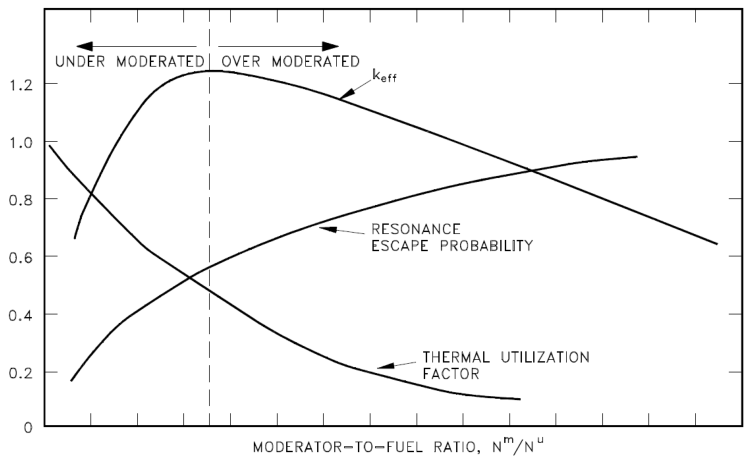
\includegraphics[width=4in]{images/dfs/under-moderation.png}
          \caption{Under Moderation Requirement} \label{um}
        \end{figure}

      \end{itemize}

\item Fast reactor considerations: we pack fuels more tightly,
  $\alpha_m > 0, \alpha_f < 0$, we use leakage to control reactivity:

  \eqn{ \frac{\derivative P_{NL}}{P_{NL}} = - \frac{L^2 B_g^2}{ 1 +
      L^2 B_g^2} \left( \frac{\dL^2}{L^2} + \frac{\derivative
      B_g^2}{B_g^2} \right) }

\begin{itemize}
\item Core flowering: fuel expands at different rate, and it would
  expand more on the top, creating a negative coefficient.

\item As temperature $\up$, number of neutrons generated per fission
  event $\up$ producing a positive feedback $\eta \up$. This is
  another positive temperature coefficient that LWRs do not have to
  worry about.
\end{itemize}


\item Power coefficient: at the end of the day, we really care about
  the power coefficient that combines fuel temperature effect and
  moderator temperature coefficient. We want the power coefficient to
  be negative.

  \eqn{ \alpha_P = \frac{\drho}{\dP} = \frac{1}{k} \frac{\pk}{\drho} =
    \frac{1}{k} \frac{\dk}{\dT_f} \frac{\dT_f}{\dP} + \frac{1}{k}
    \frac{\dk}{\dT_c} \frac{\dT_c}{\dP} }

The one reactor built that has a positive power coefficient unexpected
(designed to be -0.12mk/MW, measured at 0.28 mk/MW had to be shutdown)
is the MAPLEs medical reactor built around 2000. Fuel expands by less
than 1mm but because it is a small reactor it pushes the power
coefficient to be positive.

Key points:
\begin{enumerate}
\item Temperature defect: when we start up the reactor from CZP to
  HZP, we experience a negative reactivity due to resonances
  absorption increase:

  \eqn{ D_T = \int_{T_{\mathrm{room}}}^{T_i} (\alpha_m + \alpha_f) \dT
  }

\item Power defect: when we go from HZP to HFP, 

  \eqn{ D_P = \int_{T_i}^{T_f} \alpha_f \dT_f + \int_{T_i}^{T_c} \alpha_c \dT_c }

  where $T_c - T_i$ is fairly small ($\sim 20\degreeC$), whereas the
  power defect is dominated by the fuel materials.

\item One way we can use power defect: if for some reason we need to
  stretch out the cycle length for some, we can do coast-down by
  lowering the power, and by power defect, the reactivity would
  increase, thus we can operator for a longer period of time before
  reaching subcritical.

\item Excess reactivity: value of $\rho$ if all movable rods and
  poisons are removed from the core. We need excess reactivity to
  compensate for the temperature defect, power detect and shutdown
  margin.
\end{enumerate}

\item Reactor transients: if we assume initially critical core,
  $\alpha_m, \alpha_f < 0$. With a reactority insection $\rho(t)$, we
  can write \eqn{ \rho(t) = \rho_i(t) - |\alpha_f| (T_f(t) - T_f(0)) -
    |\alpha_m| (T_c(t) - T_c(0) ) }
\end{enumerate}


\topic{Depletion Code: ORIGIN}

This lecture was given on 10/28/13 in Lecture 15 of 22.251. 

ORIGIN is a fuel depletion and decay heat calculation code. It is very
accurate in the depletion calculation, but could be too crude (3
energy groups, 0 dimension geometry), so it is better to use ORIGIN
with a lattice code (e.g., SCALE package, CASMO, MCNP) and feed
reaction rates into ORIGIN. Sample calculation that ORIGIN can
perform:

\begin{enumerate}

\item Decay heat calculation: isotopes that dominate the decay heat: 

\begin{itemize}
\item 2.5 days: Np-239. 
\item 41 years: Cs-137, Ba-137. 
\item 740 years: Am-241, Pu-240, Pu-239. 
\item 30,000 years: Pu-239, Pu-240. 
\end{itemize}


\item Neutron \& gamma spectra: for instance, it is useful to know
  neutron and gamma energy release during shipping and storage.

\item Cask design: heat source, heat conduction, gamma/neutron transport. 
\end{enumerate}




\clearpage

\end{document}
